%% This is an example first chapter.  You should put chapter/appendix that you
%% write into a separate file, and add a line \include{yourfilename} to
%% main.tex, where `yourfilename.tex' is the name of the chapter/appendix file.
%% You can process specific files by typing their names in at the
%% \files=
%% prompt when you run the file main.tex through LaTeX.
The 5G-VINNI concept is to develop an E2E 5G facility that can be used to primarily demonstrate the practical implementation of infrastructure to support the key 5G KPIs and to accelerate the uptake of 5G in Europe by lowering the entry barrier for vertical industries to pilot use cases dependent upon those KPIs. However, 5G-VINNI is not intended to be simply a group of interconnected test facility sites as seen on Figure \ref{fig:5g-vinnimap} \cite{5gvinni-site-map} – it is underpinned by principles that will allow for highly dynamic and flexible network architectures, service deployment and testing, that will create new technical and commercial service deployment models. These will in turn drive inter-facility interconnection to enable virtualized functions from the network and service layer to be called upon from any facility, with complete location agnosticism – a truly cloud-based network instantiation that has no functional boundaries, implemented across multiple facility sites.



\newpage

\section{Architectural Principles}
\acrshort{5gvinni} is underpinned by key architectural principles identified in the \acrshort{5gvinni} proposal document. These are:
\begin{itemize}
    \item Common and consistent sets of capabilities. 
    
    All \acrshort{5gvinni} facility sites support a core set of functional components and capabilities, meaning that partners that perform trials can be assured a baseline set of capabilities at any facility.
    
    \item     Interworking between facility sites. 
    
    A key strength is the ability to perform \acrshort{e2e} testing between sites. This mandates a common set of interfaces to be supported by all facility sites to allow interaction between control plane systems and the flow of traffic.
\end{itemize}

\begin{figure}[!ht]
    \centering
    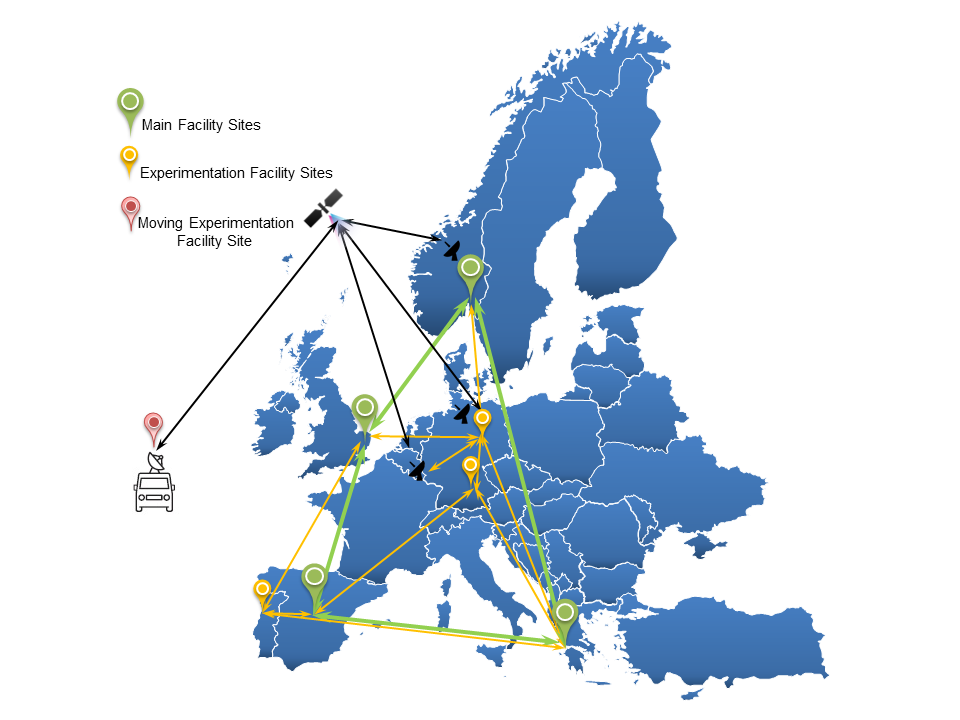
\includegraphics[width=.9\textwidth]{templates/images/chapter03/5g-vinnimap.png}
    \caption{5G-VINNI Facility with Main and Experimentation Sites. Source: \cite{5gvinni-site-map}}
    \label{fig:5g-vinnimap}
\end{figure}

\newpage
\begin{itemize}
    \item     Optional elements to support specific use cases, testing and \acrshort{kpi}s. 
    
    In order to achieve this, additional functions may be supported at sites that require them, in order to meet proprietary requirements.
    
    \item     Support for Network Slicing. 
    A key component of \acrshort{5gvinni} is the support of network slicing. This is essential for each site in order to allow simultaneous testing of multiple use cases on common infrastructure.
    
    \item     Ability for each site to evolve during the project. 
    
    5G has an underlying principle of networks built using \acrshort{vnf}s. The iterative nature of functional capabilities permits quick and with frequency changes to the network. 5G specifications is currently a work in progress and so, within the timeline of the project, standards and state-of-the-art implementations will potentially shift significantly. Therefore it is fundamental that \acrshort{5gvinni} facility sites are designed in such a way so as to allow implementations to keep pace with technological evolutions. This will maintain the \acrshort{5gvinni} facility's relevance to vertical industry partners' testing requirements throughout the duration of the project.
    
    \item     Openness and accessibility of the framework. 
    
    The design of the each facility aims to allow the flexibility and accessibility for vertical industries to run and test novel pilot use cases.
\end{itemize}
With virtualisation, orchestration and network slicing all included as underpinning architectural principles and identified as the basis for implementation as early as \acrshort{5gvinni} Release 0, it is clear that a multi-layered implementation is expected with network management and orchestration as disciplines that are pivotal for the instigation of network functions and network slices within one or multiple facility sites.

\section{Template Facility Architecture}
In the lower layer is the infrastructure, \acrshort{vnf}s and \acrshort{pnf}s in the \acrshort{ran} and Core infrastructure for the transport domain, which are expanded upon on Sections \ref{chap:vinni-ran} and \ref{chap:vinni-core-transport-infrastructure} respectively. 
Above the Network Domains, \acrshort{nfv}-\acrshort{mano} focuses on virtualization-specific tasks (i.e. management at the virtualized resource level) while domain controllers operate on non-virtualization-related operations (i.e. management at the application level). This architecture can be implemented in a range of ways, which allows individual facility sites to realize a network that can deliver a set of \acrshort{kpi}s, whilst adhering to the principles of \acrshort{5gvinni} as a whole.

    \subsection{User Equipment}
    For the most part, end-user devices are outside of the scope of \acrshort{5gvinni} as devices tend to be tied to vertical use cases and as such are in the domain of prospective ICT-19 projects. It is clear that for a device to connect to a \acrshort{5gvinni} facility site’s infrastructure, it should support reciprocal interface requirements mandated upon the \acrshort{ran}. Where required, \acrshort{5gvinni} facility sites may support devices that are specific to use cases and hence need to meet specific requirements. Theses include (but are not limited to):
    
    \begin{itemize}
        \item \acrshort{lte}-M
        \item \acrfull{nbiot}
        \item \acrfull{fwa} 
        \item \acrfull{v2x}
        \item Experimental functionality for future capabilities (R16, R17 and beyond)
        \item Air interface and connectivity testing.
    \end{itemize}
    
    \subsection{\acrfull{ran}}
    \label{chap:vinni-ran}
    Initial \acrshort{5gvinni} \acrshort{ran} architecture is aligned with what is being planned for early launches of commercial 5G networks in Europe. This will create a 5G research environment that, in some ways, closely reflects functionality and performance offered by early commercial 5G networks. Some of the \acrshort{5gvinni} facility sites may implement \acrshort{sa} architecture from start while other facilities may align with the development related to early commercial networks then migrate from \acrshort{sa} architecture during the later Releases of the \acrshort{5gvinni} project. 
    
    The \acrshort{5gvinni} \acrshort{ran} will initially offer service opportunities in the 3.5 GHz frequency band (\acrshort{3gpp} n77/n78, referred to as "mid-band") and in subsequent phases also in the 26 GHz frequency band (\acrshort{3gpp} n258, referred to as "high-band"). Specific details of what will be supported at the different facility sites depends on \acrshort{nsa} or \acrshort{sa} implementation as well as spectrum availability and device capabilities. Most notable features that need to be supported are:
\newpage
        \begin{itemize}
        
        \item \acrshort{lte} – \acrshort{nr} Dual Connectivity
        
        Dual Connectivity (EN-DC) is a mandatory part of 5G \acrshort{nsa} operation that allows early introduction of 5G by overlaying \acrshort{nr} to existing \acrshort{lte} networks connecting to the 5G enabled \acrshort{cn}.
        
        \item Uplink/Downlink Decoupling
        
        \acrshort{5gvinni} \acrshort{nsa} architecture will support uplink/downlink decoupling allowing \acrshort{lte} spectrum (using lower frequency bands than \acrshort{nr}) with superior coverage to be used for uplink traffic while \acrshort{nr} spectrum with superior peak data rate and latency is used for downlink. 
        By combining the high speed and low latency of the \acrshort{nr} downlink with the larger coverage and high reliability of the \acrshort{lte} uplink, the coverage versatility provided by \acrshort{nr} spectrum is significantly extended. 
        
        \item \acrshort{lte} – \acrshort{nr} Aggregation
        
        Increases user peak bitrates and app coverage by combining one or more \acrshort{lte} carriers with one or more \acrshort{nr} carriers to allow users to experience higher speeds in the network.
        
        \item Multiple Input Multiple Output (MIMO) 
        
        Massive numbers of antenna elements is a key feature for \acrshort{nr} systems. Especially for high frequency bands, the introduction of multi-antenna arrays enables numerous benefits. Most notably, beamforming improves data transmission coverage and link performance, while interference is minimized further improving throughput for cell-edge users.
        
        \item Numerology support 
        
        3GPP \acrshort{tr} 38.912 \cite{3GPP_TR_38.912} \acrfull{scs} enables \acrshort{ran} systems to deliver lower latency compared to legacy commercial \acrshort{lte} networks.
\newpage
        \item \acrshort{nr} Carrier Bandwidth
        
        Mid and low frequency carrier bandwidth is naturally narrower than high frequency bands. As a result, up to 100 MHz carrier bandwidth can be supported for mid-band versus 50 to 100 MHz in high frequencies\footnote{Actual implementation needs to conform with spectrum availability at the different \acrshort{5gvinni} facility site regions.}.
        
        \item Modulation
        
        64 \acrfull{qam} in uplink and downlink shall be supported, with some experimental uses of 256QAM for downlink transmission. 
        
        \item Network slice aware \acrshort{ran}
        
        For \acrshort{ran}, a network slice provides additional information on the policy for handling traffic in addition to the regular \acrshort{qos} for radio bearers.
        
        \item \acrshort{ran} integration with \acrshort{nr} Standalone (\acrshort{sa}) Core architecture
        
        When \acrshort{5gvinni} facility sites implement \acrshort{sa} architecture, \acrshort{ran} functionality shall be adopted to fulfil applicable requirements. This requires that \acrshort{ran} and UE progression needs to be aligned with the introduction of 5G Core, as this introduces new interfaces and protocols.

        \item Dynamic spectrum sharing
        
        Radio access node will dynamically determine if an \acrshort{nr} or \acrshort{lte} user is to be served, allowing NR to use the same legacy frequency bands as LTE.

    \end{itemize}
    
    \subsection{Core and Transport Infrastructure}
    \label{chap:vinni-core-transport-infrastructure}
    As previously discussed, 5G System as defined in 3GPP Rel. 15 can be realized either by 5G-\acrshort{nr} RAN connected to \acrshort{epc} (\acrshort{nsa}) or 5G-\acrshort{nr} connected to 5G Core (\acrshort{sa}). While EPC is used in \acrshort{nsa} as an evolution of the current \acrshort{lte} Core network, 5G Core is a service-based architecture with new functional nodes. 

    Transport is the part of the network that comprises the intermediate links between the CN or backbone and the sub-networks at the "edge" of the hierarchical network. Backhaul plays a vital role in mobile networks by acting as the link between \acrshort{ran} and Core.

        \subsubsection{Wireless backhaul}
        Wireless technologies operating at microwave and millimetre-wave frequencies, allow operators freedom regarding base station and small cell wireless-based backhaul. 
        
        Packet microwave or mm-wave technologies are increasingly prevalent elements of Heterogeneous Networks (HetNets), offering ample IP capacity for backhaul. \acrfull{ptp} systems can also be used as relays in a multihop backhaul network. Various topologies can be used in a backhaul deployment, depending on each specific network’s need (e.g. point-to-point line, tree structure, mesh, ring or a combination). Reliability can be achieved by using redundancy in equipment and appropriate topologies.
        In \acrshort{5gvinni}, the wireless transport network can provide a versatile solution for backhaul as a fibre substitute, as well as transport for \acrshort{iot} applications. 
        
        \subsubsection{Optical Backhaul, Midhaul and Fronthaul}
        In \acrshort{5gvinni} an optical transport solution, can be used to support backhaul, midhaul and fronthaul alternatives. Different functions in the \acrshort{gnb} result in different demand for bandwidth and latency, thus requiring different transport alternatives.

       The mid and front-haul options are currently under development (outside the scope of \acrshort{5gvinni}) and are foreseen to be integrated in the facility infrastructure along the course of the project.

        \subsubsection{Satellite backhaul}
        \acrfull{mno} likely perceive satellite backhauling services as islands of costly, difficult to integrate and inflexible connectivity. However, with the significant recent advances in satellite technology (e.g., High-Throughput Satellite) satellites can deliver cost-effective high-performance solutions to unserved and underserved areas.
        
        \subsubsection{Backhaul connectivity}
        Any backhaul connectivity deployment includes an edge node and a central node connected using a backhaul link, seen as a transport layer for the messages between the edge and the central node.
        
        The UE connects to a local terrestrial access network which is represented in this case by a 5G \acrshort{gnb}. In order to assure the connectivity to the local terrestrial access network though the different backhauls, the 5G Core Network is deployed with a functional split between the edge and central nodes.
        One of the \acrshort{nf}s associated to the backhaul connectivity architecture is the edge router which acts as a \acrfull{sd-wan} router. Data traffic is then steered according to a set of routing policies over the available backhauls previously mentioned.
        
    \subsection{Management and Orchestration}
    Management and Orchestration is a key capability for provisioning network slices. Once the underlying programmable infrastructure has been established, there is a need for components that are able to manage and orchestrate the resources within and across domains \cite{view_5g_architecture}. These functions are:
    
        \subsubsection{\acrshort{nfv} \acrshort{mano}}
        From a resource management point of view, services are deployed and operated as \acrshort{nfv} NSs. With \acrshort{nfv} \acrshort{mano}, facility operators are able to deploy and execute services in the \acrshort{nfvi} with great agility and flexibility. The \acrshort{nfvi} in \acrshort{5gvinni} facility spans across the seven facility sites and consists of different PoPs for \acrshort{vnf} deployment and execution, ranging from cell sites to regional DCs. 
        Each facility site will have its own \acrshort{nfv} \acrshort{mano} stack to manage and orchestrate \acrshort{nfv} NSs within its administrative domain while exposing a set of SBIs and NBIs to facilitate the interaction with the rest of facility site components. 
        The stack deployed at each facility site has three types of functional blocks (NFVO, VNFM, and \acrshort{cim}) and four data repositories (NS Catalog, \acrshort{vnf} Catalog, \acrshort{nfv} Instances Repository, and \acrshort{nfvi} Resources Repository). This guarantees interoperability across \acrshort{5gvinni} facility sites at \acrshort{nfv} level, regardless of any implementation-specific issues. The fact that \acrshort{etsi} \acrshort{nfv} defines \acrshort{nfv} \acrshort{mano} stack as a reference framework not only allows network operators and vendors to implement its components using open source or vendor specific solutions but also introduce some architectural modifications.
        
        \subsubsection{Network-Domain Controllers}
        \begin{enumerate}
            \item \acrshort{ran} and Core Domain Controllers
            
            The Domain Controllers at the \acrshort{ran} and Core are in charge of managing the different \acrshort{nf}s at the application level (independently of their deployment), and in general to provide control on all the non-virtualization-related operations. Core \& \acrshort{ran} domain controllers can be mapped to the EMS function group of FCAPS (Fault, Configuration, Accounting, Performance and Security management) for the functional/application part of the underneath deployed \acrshort{pnf}s and \acrshort{vnf}s. In this way we can say that these domain controllers perform changes at the application level in a “vertical” way on functions “horizontally” deployed by the NFVO.
            
            \item Transport Domain Controllers
            
            The Domain Controllers at the transport include components such as SDN controllers or \acrshort{mpls} management and control components. In \acrshort{5gvinni} the Transport network will provide advanced backhaul functionality, to interconnect for instance different locations from a common site.
            \acrshort{mpls} networks for instance are well-known solutions used for several years in the transport network. \acrshort{mpls} allows the visualization of the \acrshort{e2e} path instead of a hop by hop vision.
            
            \begin{figure}[!ht]
                \centering
                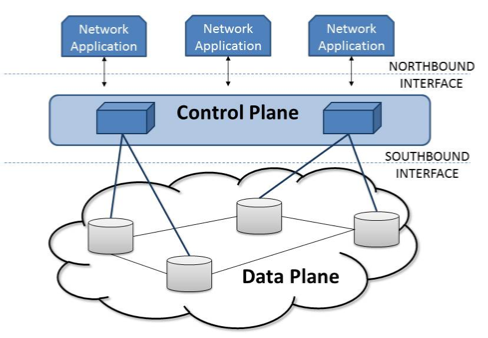
\includegraphics[width=.9\textwidth]{templates/images/chapter03/sdn-architecture.png}
                \caption{SDN Architecture According to IETF RFC 7426. Source: \cite{view_5g_architecture}}
                \label{fig:sdn-architecture}
            \end{figure}  
            
            The \acrshort{cp} and the data plane are separated from each other. In addition, the \acrshort{cp} is logically centralized in a software-based controller defined as the “network brain”, while the data plane is composed of network devices (“network arms”) that forward packets. The \acrshort{cp} includes both northbound and southbound interfaces. The northbound interface provides a network abstraction to network applications, and the southbound interface (e.g., OpenFlow) standardizes the information exchange between the control and data planes \cite{rfc7426}.
            
        \end{enumerate}

        \subsubsection{\acrshort{e2e} Service Operations and Management}
        \acrshort{e2e} Service Operation and Management, within the \acrshort{5gvinni} architecture, encompasses the management and operations of \acrshort{e2e} services that span multiple domains. It translates service design into configuration of resources (physical and virtualized) needed for service establishment. Using orchestration to coordinate between domain controllers and \acrshort{nfv}-\acrshort{mano}, \acrshort{e2e} services may span multiple network domains provided by different administrative entities (e.g., different network service providers or external partners).
        Effectively, \acrshort{e2e} \acrshort{mano} connects the business needs of verticals to the resource and network capabilities exposed by management and partner provider domains. It thereby enables orchestration and management across multiple domains, doing so by offering customer facing services northwards via standardised API’s to fulfil service requirements. The \acrshort{e2e} \acrshort{mano} translates business services into their corresponding component network services and requests the services from the appropriate domain. In this way the \acrshort{e2e} \acrshort{mano} abstracts how the business services are realised at the resource level, thereby allowing verticals to focus on their Service Level Agreements (SLAs) rather than the service implementation itself.

    \subsection{Security, Testing and Monitoring Architecture}
    With the use of \acrshort{nfv} and SDN in 5G, one of the main priorities is for a secure cloud environment between tenants and slice instances. Security needs to be present in all sub-domains of the cloud to address the current threat landscape with sophisticated actors, adhere to privacy and security regulations in the different markets and ensure isolations of tenants and network slices. The main security controls that need to be established in the cloud domain are:
    \begin{itemize}
    \item Infrastructure network zoning model that applies to all layers of the infrastructure.
    \item Solid multi-tenancy capabilities through the infrastructure platform.
    \item Security monitoring through flow based network analytics.
    \item Centralized logging with analytics capabilities.
    \item Server integrity checking and configuration auditing.
    \end{itemize}
    Note that there are other important security functions, such as DDoS protection, Intrusion Detection and Prevention Systems (IPS/IDS), antivirus, antimalware etc. The aim is not to cover all security requirements and features in this section. In the following, briefly described are architectural principles for the zoning model and multi tenancy.

        \subsubsection{Zone Model}
        The infrastructure network zoning model is fundamental in addressing the shared technology challenge in a multi-tenant platform. The defined zone model regulates how the cloud infrastructure is built and how segmentation is achieved.
        A security domain is an entity that defines the level of control and governance present; it does not itself have any policies, but exists to define where boundaries are present. A domain can consist of one or more security classes. Security domains defined in level of trust are: un-controlled, controlled, restricted, secure, and externally controlled domain with traffic not allowed to flow directly between non-adjacent domains. Security Zone Classes is a concept of aggregating network zones with the same exposure and security levels. Traffic from one security class to another will need to pass two different layers of security with one being logical or virtual and with the second layer being physical.

        \subsubsection{Multi-tenancy}
        Multi-tenancy enables separation between tenants running services in a shared environment. In a multi-tenant deployment, the resources controlled by one tenant are physically or logically separated and secured from other tenants. Multi-tenancy is a key requirement for services across both public and private cloud environments.

    The testing architecture has a purpose that is primarily establishing automation services that encompasses every phase of the infrastructure deployment. Nowadays, this is considered a very important stage given the number of performance and interoperability variables at stake in modern virtualized systems. The second purpose of the testing infrastructure is to provide testing and experimentation services to the vertical service operators but also to the mobile operators themselves for network maintenance purposes. This is a fundamental step for ensuring reliability, resilience, and performance of the slice components and of the slice as a whole during the slice deployment phase, a due process before handing the slice over to the customer. Such system is used to monitor all the components, from the virtualised infrastructure to the Quality of Experience (QoE) of the traffic carried by the network. While its presence would be highly suggested, the complexity of virtualized networks make a full monitoring extremely heavy and resource-demanding.

\section{Interconnection and Interoperability of sites}

    \subsubsection{Interconnection Between Sites}
    This section explains the architectural requirements in terms of connectivity between sites. As a main principle, it is important that all sites have IP connectivity with each other. For such purpose, each site shall have one or more facility site gateways (FSGW) that fulfils the following requirements. In the long term solution, two FSGWs can be preferred for increased load balancing and resilience capabilities. 
    
    \begin{itemize}
        \item Public IP.
        \item Routing protocols, especially exterior gateway protocols, such as Border Gateway Protocol (BGP).
        \item Generic Routing Encapsulation for the establishment of GRE Tunnels.
        \item Internet Protocol Security (IPsec) protocol suite.
    \end{itemize}
    For \acrshort{qos} Differentiation on the connection between sites the following options are under evaluation. 
    \begin{itemize}        
        \item Best Effort Internet\footnote{In the initial phase, all sites will use Best Effort internet. However, the possibility that the connection between some specific pair of sites will be upgraded gradually to \acrshort{mpls}-\acrshort{vpn} and/or \acrshort{sd-wan} with \acrshort{mpls} Core is under evaluation.}.
        \item \acrshort{sd-wan}, where the traffic can be sent over a combination best-effort Internet paths and some way of using \acrshort{mpls} Core or direct DiffServ-enabled traffic exchange between the operator domains.
    \end{itemize}
    
    This will enable SD-WAN for \acrfull{asq} interconnection paths between sites and value added connectivity (VAC) triggered and handled on-demand for end-point traffic flows whose traffic can be steered. For the support of use cases and scenarios beyond the basic service offerings (based on best-effort Internet interconnection) the support for enterprise \acrshort{vpn} is a viable alternative. These services can be relevant for enterprise customers managing their applications as tenants or connecting to partner enterprises that operate as tenants of one or more facility sites. 
    
    Some characteristics of the \acrshort{mpls} and \acrshort{sd-wan} concepts are:
    \begin{itemize}
        \item Classic \acrshort{mpls} \acrshort{vpn} with \acrshort{qos}
        
        \acrshort{mpls} is a very well-known connectivity solution. With \acrshort{mpls}, the operator can make separate bandwidth reservations for different classes of traffic and give different forwarding behaviour based on the class \cite{4287988}.
    
        \item \acrshort{sd-wan} with \acrshort{mpls} Core
        
        This concept uses software-defined networking in a Wide Area Network (WAN), and is based on the traditional \acrfull{sdn} principle of separating the \acrshort{cp} from the data plane. One of the advantages that it offers is to enable the use of private WAN connections such as those based on \acrshort{mpls} with conventional internet access. \cite{7939138, 8308427}
    \end{itemize}

    \subsubsection{Interoperability Between Sites}
    Once the different \acrshort{5gvinni} sites are interconnected as presented in the previous section interoperability is in order for network services to be deployed and operated across said sites.
    
    \begin{figure}[!ht]
        \centering
        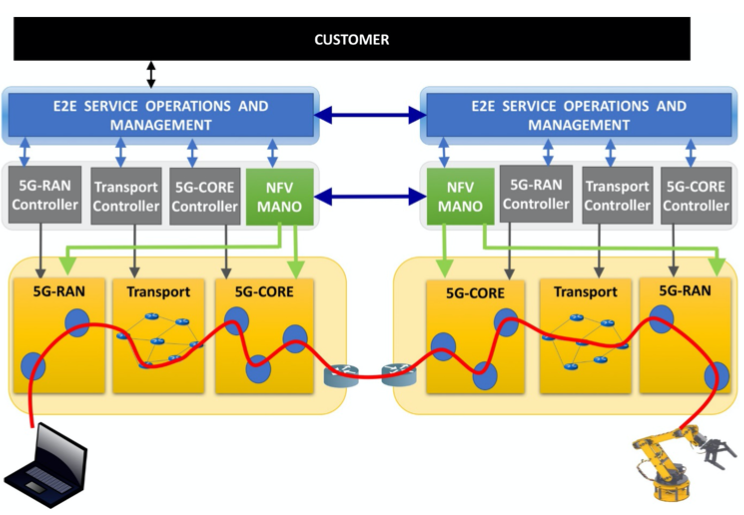
\includegraphics[width=.9\textwidth]{templates/images/chapter03/service-inter-operation.png}
        \caption{Service Inter-Operation across \acrshort{5gvinni} Sites. Source: }
        \label{service-inter-operation}
    \end{figure}  
    
    In order to enable such interoperability, the use of north-south bound and east-west bound interfaces are needed in order to guarantee the proper understanding of the service needs on each of the involved sites. While the arrows are here drawn directly to and from the \acrshort{nfv} \acrshort{mano} in the neighbour domain this will typically be realized via inter-provider \acrshort{api}s\footnote{In this regard, it is important to note also that the specifications of these inter-provider \acrshort{api}s are still at an early stage and to be considered as a key activity and work in progress by the industry forums and specification defining organizations.} (e.g. along the lines of 5GEx Project \cite{carlos_bernardos_2016_671636}).

\subsection{5G Network Slice Federation Scenarios}
This section presents two types of Network Slice Federation Scenarios. First is how an \acrshort{e2e} 5G Network slice federation is created involving Access, Transport and Core by presenting a paradigm of another project, namely the 5GinFIRE H2020 project \cite{5ginfire} and how it can be adapted for other research projects. The second presents how an \acrshort{e2e} 5G Service Level Federation can be deployed with an \acrshort{e2e} cross-domain orchestrator between facilities.
    
    \subsubsection{Network Slice Federation Across \acrshort{5gvinni} Facility Sites}
    An example scenario of \acrshort{e2e} network slice federation across three different \acrshort{5gvinni} Facility Sites is illustrated in Figure \ref{fig:e2e-deployed} which involves three facilities (e.g., Norway Site, UK Site and Spain Site) providing a single \acrshort{e2e} network slice.
    
    \begin{figure}[!ht]
        \centering
        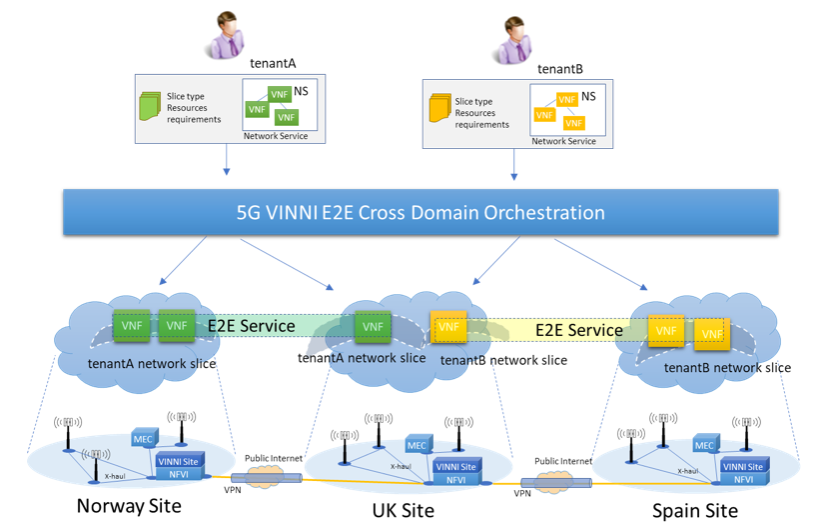
\includegraphics[width=0.9\textwidth]{templates/images/chapter03/e2e-deployed.png}
        \caption{\acrshort{e2e} Network Slice Federation across three different Facility Sites. Source: }
        \label{fig:e2e-deployed}
    \end{figure}
    
    In order to have such a scenario as per Figure \ref{fig:e2e-deployed}, the facilities would need to have established agreements in the business (e.g. what type of resources are allowed and at what cost) and connectivity level (e.g. Layer 2 or 3). With respect to the latter, related work of such deployment has been done by 5GinFIRE \cite{5ginfire} where a single \acrshort{mano} is responsible for orchestrating multiple interconnected and physically separated \acrshort{nfvi}s. In \acrshort{5gvinni}, however, each facility has its own \acrshort{mano} stack. 
    
    In 5GinFIRE, partner testbeds have mutual agreements in regards to joining and accepting NFs and also allowing access of their \acrshort{vim}'s \acrshort{api}s to a centralized \acrshort{mano}. This cross-site interconnectivity supports the exchange of control and data-plane information among sites, utilizing an overlay of a network architecture based on \acrshort{vpn}s. This approach \cite{diego_lopez_2018_732497}, given that sites are physically separated at different network locations, means that inter-site communications may traverse multiple untrusted network domains. Inter-site data-plane communications will require the creation of specific \acrshort{cim} networks at each site, with network connectivity towards the appropriate \acrshort{vpn} endpoint of the site. These networks will then be used to attach any \acrshort{vnf}s needing this type of communications, while guaranteeing all subsequent security principles. 
    
    \subsubsection{Service Level Federation across \acrshort{5gvinni} Facility Sites}
    In these scenarios, two \acrshort{5gvinni} facility sites support different types of network slices in order to create an \acrshort{e2e} service for \acrshort{5gvinni} customers. Although the federation can be seen at the Service Layer, the interconnection and interworking between the two slices would be required to support \acrshort{e2e} service operation.
  
    \begin{figure}[!ht]
        \centering
        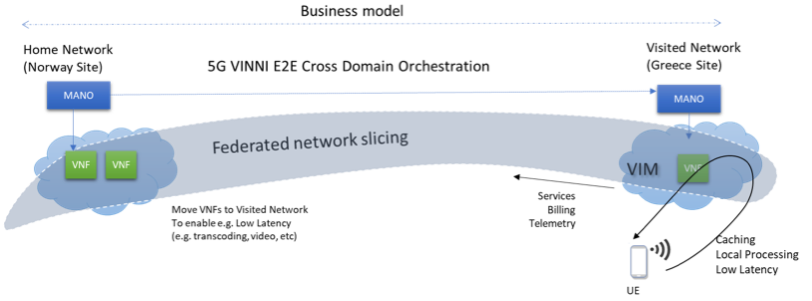
\includegraphics[width=0.9\textwidth]{templates/images/chapter03/mult-tenants.png}
        \caption{Multiple Tenants and Federated Network Slicing. Source: }
        \label{fig:multiple-tenants}
    \end{figure}     
    
    Figure \ref{fig:multiple-tenants} displays a generic view of how multiple tenants can use the \acrshort{5gvinni} \acrshort{e2e} Facility to deploy an \acrshort{e2e} service on top of a network slices types. This connectivity provides a unified service experience for the creation and roaming extension of network slices optimized for demanding scenarios. Today such scenarios are exclusibely enabled for cloud services, but with the introduction of network slice requirements, services must move to the edge. In order to ensure the performance demands, edge processing is necessary to maintain latency within limits and make sure the 5G application behaves as usual, even in roaming scenarios.

%\section{Facility-Site: Greece}
%    
%    \subsubsection{Radio Access Network (\acrshort{ran})}
%    
%    LimeNET Mini is based on Mini-PC Barebone (BRIX) platform complete with an integrated LimeSDR USB with added shielding. 
%    The hardware is fully qualified for compatibility with the LimeNET Ubuntu app store. This allows Patras University and project partners to create and deploy applications to configure the system for 5G applications with no system compatibility issues.
    
%    LimeNET Base station is a software defined radio power house. It is based on top of the line PC fitted with the newly developed LimeSDR QPCIe board. This new board is a much more sophisticated version of the LimeSDR board used in LimeNET Mini. It has two LMS7002 transceiver chips instead of one, which allows for a 4x4 MIMO configuration instead of a 2x2 MIMO configuration.
    
%    SRS primary role consists of setting up the software side of the Patras \acrshort{ran} Facility. This will include deploying a 4G software-defined network using the currently available open-source srsUE, srseNB and srsEPC products, and designing and implementing new 5G \acrshort{nr} solutions. The latter effort will span the duration of the whole project. Next, we list the several solutions SRS plans to make available and accessible in the Patras Facility by the final release of \acrshort{5gvinni}:
%    \begin{itemize}
%        \item srsUEs - software-defined \acrshort{lte} \acrshort{ue}s, capable of performing 2x2 MIMO, carrier aggregation, multicast, and handover. The srsUE will be available in the outdoor and indoor testbeds. In the outdoor testbed, it will run on LimeNET mini boards equipped with power amplifiers to sustain long distance connections. In the indoor testbed, the srsUEs will run on LimeSDR minis, with all the baseband processing performed in a laptop. 
        
%        \item srseNB - software-defined \acrshort{lte} eNB. The srseNB is currently capable of performing MIMO, multicast, and different scheduling algorithms. It will run on a LimeNET Base Station in the Patras outdoor testbed, and on a Lime SDR mini connected to a laptop in the indoor testbed.
        
%        \item srsgUE - software-defined Non-Standalone (\acrshort{nsa}) gUE, including the 5G \acrshort{nr} PHY and upper layers. It is currently in a stage of early development.
        
%        \item  srsgNB - software-defined Non-Standalone (\acrshort{nsa}) \acrshort{gnb}, including the 5G \acrshort{nr} PHY and upper layers. It is currently in a stage of early development.
%    \end{itemize}

%    Edge site is planned for Rel-1. The decision on location is not yet decided and will depend on requirements of the funded ICT-19 projects. 
%    Nevertheless, the Edge site will be included with one of the solutions presented in next figure: Either the Edge site compute nodes will be managed by OpenStack, or the Edge site will be seen as its own \acrshort{cim}, handled as a multiVIM scenario by \acrfull{osm} deployed at Patras Facility-site

%    \subsubsection{Core}
%    The 5G Mobile Core is realized by the deployment of Fraunhofer FOKUS' Open5GCore. Open5GCore is a use case-agnostic, standard compliant software-only prototype, implementing the 5G Core components and interfaces, addressing the use cases of seamless mobile broadband connectivity, multimedia and content delivery and massive \acrshort{iot}. For more details on Open5GCore please refer to the Berlin Facility-site description of this chapter. 

%    \subsubsection{Transport Infrastructure}
%    The transport network that will connect the \acrshort{ran} with the Core in the Patras Facility-site, will consist of the following connections: 
%    \begin{itemize} 
%        \item The Facility will be interconnected via a dedicated 10 Gb link with GRNET NRN in Athens that will allow high speed connectivity to public Internet but also to dedicated GEANT links or \acrshort{vpn} connections with other \acrshort{5gvinni} sites.
%        \item Point-to-Point mmWave wireless links, operating at 71-76/81-86 GHz and delivering up to 10 Gbps, will interconnect the University campus with selected sites several kilometres away, backhauling the gNBs and FWA that will serve public places in Patras sub-urban area.
%        \item Fixed Wireless Access (FWA) links at 26/28 GHz bands, providing up to 1 Gigabit Ethernet to the subscriber and up to 1.6 Gbps aggregate capacity per sector, will interconnect two buildings of public interest in Patras sub-urban area, providing access to \acrshort{5gvinni} core network services.
%    \end{itemize}
    
%    \begin{figure}[!ht]
%        \centering
%        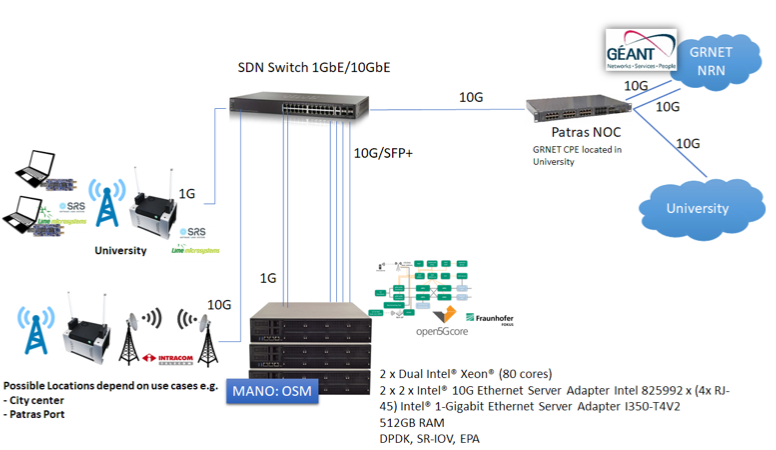
\includegraphics[width=0.9\textwidth]{templates/images/chapter03/fwa-backhaul-patras.png}
%        \caption{FWA and Backhaul Networks at Patras Facility-Site}
%        \label{fig:fwa-backhaul-patras}
%    \end{figure}
    
%    Detailed radio planning studies has been performed to identify the optimum locations, the appropriate equipment and its configuration, to provide high-speed fixed wireless access to two public services establishments, and to cover this, along with a collocated \acrshort{gnb}, with high capacity, low latency, long range backhaul. The results of these studies are listed in the LLD of the Facility.
    
%    \subsubsection{Management and Orchestration}
%    The Patras Facility uses currently OSM FOUR but will migrate to Open Source \acrshort{mano} version FIVE with OSM FIVE VNFM support 
%    \acrshort{osm} is an \acrshort{etsi}-hosted open source community delivering a production-quality \acrshort{mano} stack for \acrshort{nfv}, capable of consuming openly published information models, available to everyone, suitable for all \acrshort{vnf}s, operationally significant and \acrshort{cim}-independent. OSM is aligned to \acrshort{nfv} ISG information models while providing first-hand feedback based on its implementation experience.

%    A first approach towards this is to use the existing work from 5GinFIRE project [21] and mainly integrate for the Release 1 the 5GinFIRE portal to deploy NSs. Within 5GinFIRE some of the core functionalities that facilitate the LCM of various artefacts have been defined:
    
%    \begin{itemize}
%        \item Management of \acrshort{vnf}s, NSDs, users, infrastructures and experiments in portal
%        \item Maintain a reusable public catalog of \acrshort{vnf}s and NSDs together with versioning, licensing, etc
%        \item Description and availability of experimentation resources
%        \item Onboarding/Offboarding \acrshort{vnf}s/NSDs to multiple MANOs
%        \item Validation of \acrshort{vnf}s, NSDs
%        \item \acrshort{vnf}s Images management: These repositories contain the \acrshort{vnf} images that need to be deployed in target \acrshort{vim}s
%        \item Experimentation scheduling and deployment requests as well \acrshort{vnf} placement to multiple \acrshort{vim}s for distributed Network Services
%    \end{itemize}
    
%    \subsubsection{Security}
%    All Patras Facility infrastructure will have its own private network. The \acrshort{nfvi} infrastructure is behind a firewall with restricted access to Internet allowed only to specific services.

\newpage    
    \subsection{Use Case Verticals} 
    \label{chap:ucv}
    The \acrshort{5gvinni} facility site in Patras (Greece) will be an exemplary Open Source 5G-\acrshort{iot} facility. This means that most of the installed components will be offered as Open Source but there will be also dedicated components and services to support 5G-\acrshort{iot} scenarios. Numerous partners will deploy their technologies in the Patras/Greece facility, thus creating a unique 5G playground for \acrshort{kpi} validation and support on future verticals. 

    \subsubsection{Verticals Summary}
    Additionally, please note that these use cases could be combined and create different scenarios, by using some aspects of each distinct use cases.
    The service offerings referred in the Greece portfolio are detailed in Table \ref{tab:service-offerings} including information on their service exposure level and their ability to support the aforementioned use cases.

    \begin{table}[!ht]
       \begin{threeparttable}
    \caption{Service Offerings in the Greece Portfolio}
    \label{tab:service-offerings}
    \setlength\tabcolsep{0pt} % make LaTeX figure out intercolumn spacing
    
    \begin{tabular*}{\columnwidth}{@{\extracolsep{\fill}} lll}
    \toprule
         Service offerings & Service exposure & Supported use cases\\
    %     \multicolumn{4}{c}{Accuracy (\%)} \\ 
    %\cmidrule{3-6}
    %     & & K3 & K6 & L1 & mean\tnote{c} \\
    \midrule
          \acrshort{embb} network SaaS & Level 3-4 & UC1\tnote{1}, UC2, UC4 \\
    \addlinespace
         uRLLC network SaaS & Level 3-4 & UC1\tnote{1} \\
    \addlinespace
          mIOT network SaaS & Level 3-4 & UC3 (\acrshort{iot} slicing) \\
    \addlinespace
          Customised network slice & Level 3-4 & UC1\tnote{1}, UC3 (NB-\acrshort{iot} slicing) \\
    \bottomrule
    \end{tabular*}
    
    \smallskip
    \scriptsize
    
    \begin{tablenotes}
    \RaggedRight
    \item[1] Due to uRLLC and \acrshort{embb} characteristics, the UC1 should be executed in a customised network slice. Until this service offering becomes available in the Greece portfolio, UC1 will be executed (with some limited performance and/or functionality) in \acrshort{embb} and uRLLC network slices offered as a service to the CSC.
    \end{tablenotes}
       \end{threeparttable}
    \end{table}
    
    In Greece facility site, the following use cases are selected as the main candidates for \acrshort{5gvinni} validation purposes:
    
\newpage
    
    \subsubsection{UC1 – First Person View Remote Control Vehicle (Automotive)}
    This use case consists of a remote-controlled vehicle with an on-board camera that provides real-time video streaming, allowing for remote operating. The camera provides real time frontal view of the vehicle, so the user can steer the vehicle by means of a controller. The video streaming aspect of the use case requires a significant amount of data received through the 5G network, while the remote-control aspect requires low latency and high reliability delivery of the movement commands. To satisfy these requirements, capabilities provided by \acrshort{embb} and \acrshort{urllc} slices are critical.
\medskip
    \begin{figure}[!ht]
        \centering
        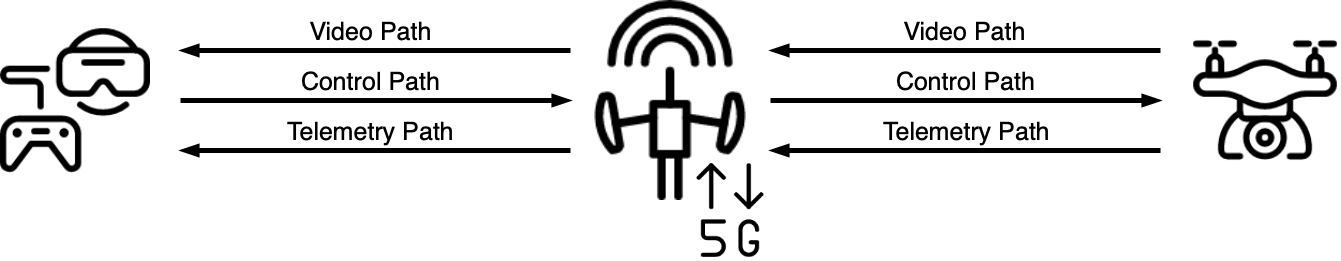
\includegraphics[width=0.9\textwidth]{templates/images/chapter03/use-case-01.png}
        \caption{Greece UC1 – First Person View Remote Control Vehicle Use Sase}
        \label{fig:uc1}
    \end{figure}     

    \subsubsection{UC2 – 360-degree Video broadcast (Media and Entertainment)}
    This use case involves video streaming with a 360-degree camera. A possible scenario is during Patras carnival festivities, where participants can be equipped with 5G-enabled devices with 360o cameras in order to transmit the local festivities to remote locations while being able to move around downtown Patras. The main requirements of this use case are high throughput and high connection density in crowded scenarios. 
\medskip
    \begin{figure}[!ht]
        \centering
        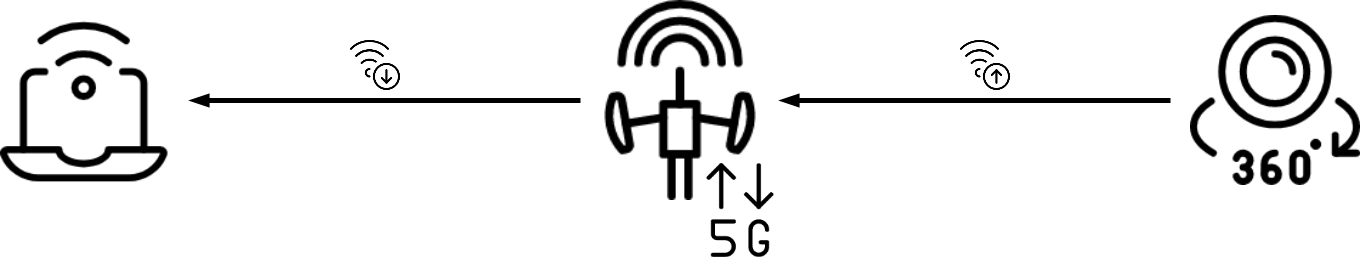
\includegraphics[width=0.9\textwidth]{templates/images/chapter03/use-case-02.png}
        \caption{Greece UC2 – 360\degree Video Broadcast Use Case}
        \label{fig:uc2}
    \end{figure}  	
\newpage
	\subsubsection{UC3 – NB-\acrshort{iot} Coverage and \acrshort{iot} Slicing study}
	The suggested use case for NB-\acrshort{iot} consists of two phases. In the first phase, a coverage study of NB-\acrshort{iot} devices will be carried out on the University of Patras (see Figure \ref{fig:uc3}). In this study, a large number of NB-\acrshort{iot} devices will be deployed and the network coverage will be examined, taking into consideration various factors including (but not limited to) distance from the antenna and penetration power. Once these factors have been analysed, then the second phase will apply the concept of \acrshort{iot} slicing, making use of distinct \acrshort{iot} applications provided by corresponding virtualized \acrshort{iot} Gateway instances deployed in separated \acrshort{nsi}s (see Figure \ref{fig:subim2}).
\medskip
    \begin{figure}[!h]
        \begin{subfigure}{\linewidth}
            \centering
            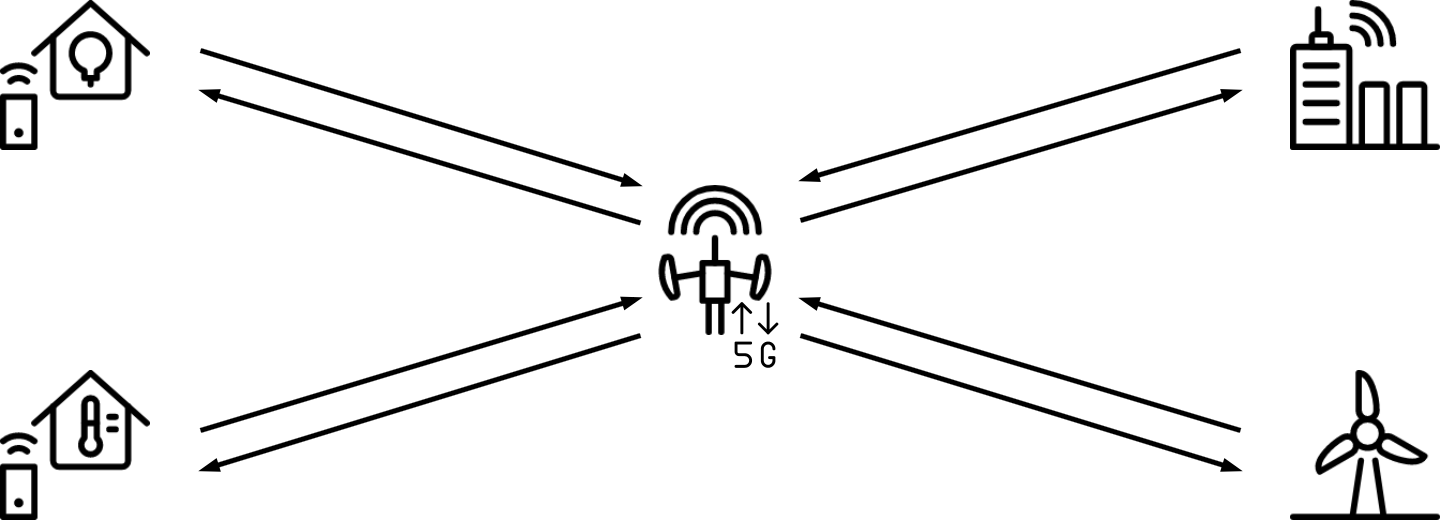
\includegraphics[width=0.9\linewidth]{templates/images/chapter03/use-case-03.png} 
            %\captionsetup{width=.9\linewidth}
            \caption{Greece UC3 – NB-\acrshort{iot} Coverage}
            \label{fig:uc3}
        \end{subfigure}
        %\hspace{10pt}
        \hfill
        \begin{subfigure}{\linewidth}
            \centering
            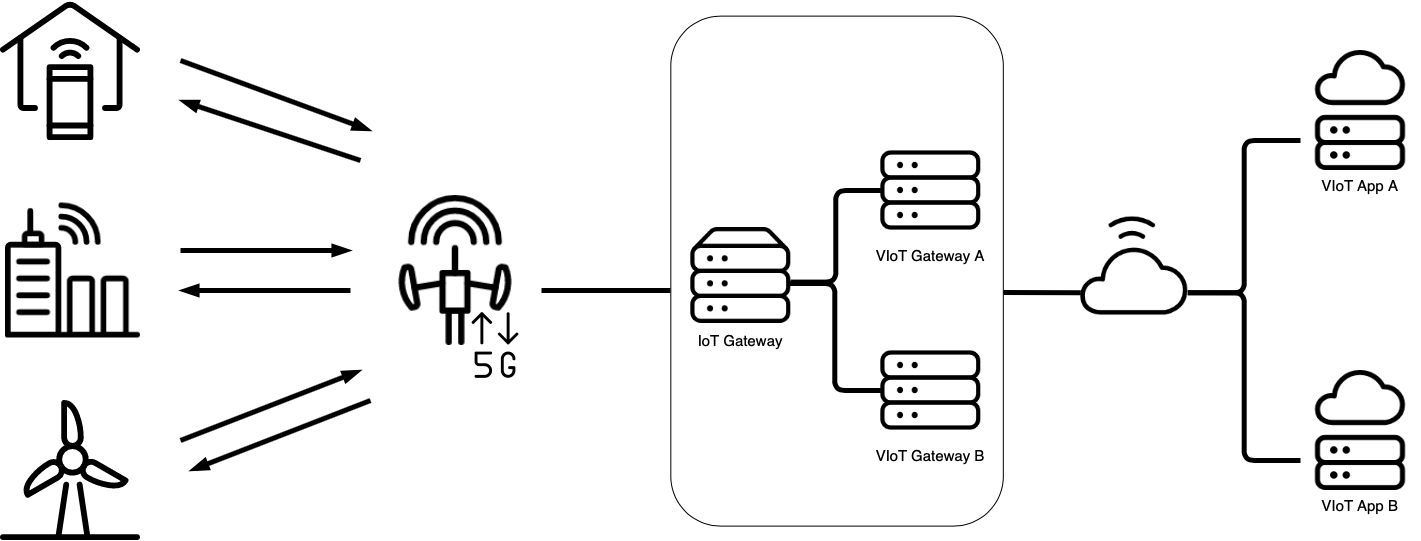
\includegraphics[width=0.9\linewidth]{templates/images/chapter03/iot-slicing-concept.png}
            \caption{Greece UC3 – Concept of \acrshort{iot} Slicing}
            \label{fig:subim2}
        \end{subfigure}
        \hfill
        \caption{Greece UC3 - Narrowband IoT Use Case}
        \label{fig:iot-slicing-concept}
    \end{figure}
\newpage	
	\subsubsection{UC4 – \acrshort{ar} Use Case (Media and Entertainment)}
	This use case describes the delivery of \acrshort{ar} annotations on top of a video stream captured by an end user of the service. The end user captures video, which is delivered to an \acrshort{ar} application backend responsible for object recognition, tracking and annotation of the video with related information. The video annotation is performed taking into account the position of the identified objects in the video and delivered as an enhanced video stream to the user. This scenarios’ main requirement is the very high throughput. To satisfy these requirements, the operator of this use case may rely on the communication capabilities provided by an \acrshort{embb} slice. This use case is expected to be supported by DFKI, as a member of the Executive Board. The exact application context will be later defined, choosing from the wide DFKI portfolio. A candidate application targets the touristic domain, providing informational annotations on top of identified monuments. The use case targets the use of a \acrshort{mec} location within the Patras facility, as a means to lower latency. 
\medskip
    \begin{figure}[!ht]
        \centering
        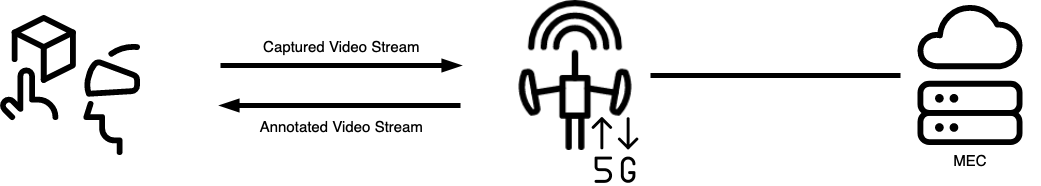
\includegraphics[width=0.9\textwidth]{templates/images/chapter03/use-case-04.png}
        \caption{Greece UC4 – \acrshort{ar} Use Case}
        \label{fig:uc4}
    \end{figure}